\documentclass[12pt]{article}
\usepackage{geometry}
\geometry{letterpaper, left=22.5mm, right=22.5mm, top=30mm, bottom=30mm}
\geometry{letterpaper}
\usepackage{amsmath}
\usepackage{amssymb}
\usepackage{enumitem}
\usepackage{fancyhdr}
\usepackage{framed}
\usepackage{tikz}
\usepackage{mathpazo}
%\usepackage{charter}
%\usepackage{newcent}
\usepackage{indentfirst}
\usepackage{booktabs}
\usepackage{graphicx}
\usepackage{float}
\usepackage{makecell}
\usepackage{xcolor}
\usepackage{mdframed}
\usetikzlibrary{trees}
\pagestyle{fancy}
\usepackage{amsthm}
\theoremstyle{definition}
\newtheorem{definition}{Definition}[section]
\theoremstyle{property}
\newtheorem{property}{Property}[section]
\theoremstyle{assumption}
\newtheorem{assumption}{Assumption}[section]
\theoremstyle{example}
\newtheorem{example}{Example}[section]
\theoremstyle{comment}
\newtheorem{comment}{Comment}[section]
\newtheorem{theorem}{Theorem}[section]
\newtheorem{corollary}{Corollary}[theorem]
\newtheorem{lemma}[theorem]{Lemma}
\usepackage{lastpage}
\usepackage{wrapfig}
\usepackage{hyperref}
\usepackage{subcaption}
\usepackage{setspace}
\hypersetup{
colorlinks=true,
linkcolor=black,
filecolor=green, 
urlcolor=blue,
}
\newcommand{\ROM}[1]
    {\MakeUppercase{\romannumeral #1}}
\fancyhead[L]{Econometrics \ROM{2}: Recitation 13 }%change each reci
\fancyhead[R]{Spring 2020}
\fancyfoot[C]{\thepage \hspace{1pt} / \pageref{LastPage}}

\fancypagestyle{firstpage}{%
\fancyhf{}%
\renewcommand{\headrulewidth}{0mm}%
  \fancyfoot[C]{\thepage \hspace{1pt} / \pageref{LastPage}}
}
%change title each rec
\title{Introduction to Econometrics \ROM{2}: Recitation 13\footnote{This is based on the lecture notes of Professors Jushan Bai and Bernard Salanie. I was also greatly helped by previous recitation notes from Paul Sungwook Koh and Dong Woo Hahm. The remaining errors are mine. }}

\begin{document}
\linespread{1.25}
\onehalfspacing

\author{Seung-hun Lee\footnote{Contact me at \href{mailto:sl4436@columbia.edu}{sl4436@columbia.edu} if you spot any errors or have suggestions on improving this note.}}
\date{Undated}
\maketitle
\thispagestyle{firstpage}

%%%%%%%%%%%%%%%%%%
\section{Machine Learning}
\subsection{Random Forests}
Random forests use a series of decision trees - a stack of two-way splits with several number of depths - to solve a classification problem. The splits are based on covariate $k$ being above or below a certain threshold. The process stops at some depth and predict with the mean of $y$ at the terminal node $x$ belongs to. The covariate and the threshold combination that determine the split are selected so as to have the largest separation possible. This is commonly referred to as a `greedy' way of creating random forests.  \par
The detailed way of constructing random forests are as follows. Randomness is injected in several levels: one to select a random sample to train each tree on. Second level of randomness is involved in selecting variable candidates to determine splits for the trees. At the end, we get a prediction for any $x$, average of the predictors of the trees. We can also estimate the prediction error at any observation $x_i$ and gain expected prediction error overall. We can also identify which covariates contributed the most the the prediction using the variance-importance plots. This is where the random forests gain the advantage of interpretability - explaining as to why the results of the prediction came out to be as it is (not just spitting out the number). \par
There are some trade-offs. We want some level of depths in order to reduce the variance in the prediction and get a better fitting. However, too much depth will lead to overfitting. It is usually very difficult to find the happy medium. \par
Below is the example of the decision brought from Varian (2014). A random forests would be obtained by multiple trees, each with different sample (selected through bootstrap) and different variable and threshold combination. 
\begin{figure}[H]
\centering
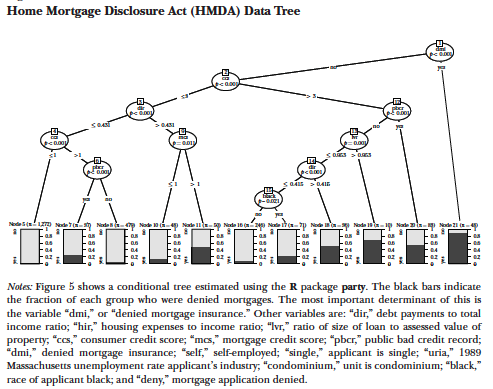
\includegraphics[width=0.7\textwidth, keepaspectratio]{randomforest.png}
\caption{From Varian (2014), Figure 5}
\end{figure}\par
\subsection{Double Machine Learning De-biasing Technics}
Often we are interested in testing for regarding the value of the parameter of interest. For instance, the average treatment effect under the conditional independence assumption. Specifically, we assume $(\epsilon_i(1),\epsilon_i(0))\perp\!\!\!\perp u_i|X_i$ where $X_i$ contains a large set of covariates. What we may do is to estimate the propensity score using machine learning techniques such as LASSO. Then, estimate the average treatment effect with the formula of our choice. Ideally, we want to conduct some standard tests. \par
Here is the problem - what we have for the propensity score is an estimate with some error. So depending on the size of this error, the estimate of the average treatment effect could be affected. Moreover, the propensity score is just a means towards our ultimate goal of obtaining the average treatment effect - it is merely a nuisance parameter. Since what we are doing involves errors at two different stages, we need a double machine learning de-biasing technics. Specifically, we decouple the propensity score and the treatment effect by applying Neyman Orthogonalization. In principle, what this method allows us to do is to do a two-step estimation by getting the estimate for the propensity score and then estimate the ATE without having to worry too much about the contaminated standard errors originating from the fact that we are not using the exact the propensity score. \par
In our case, what we can do is to
\begin{enumerate}
\item Split data into $K$ folds
\item Use LASSO to estimate $\hat{P}_k=\Pr(D_i=1|X_i)$ in all folds except the $k$th one. $k$ can be from 1 to $K$. 
\item If we are using inverse probability weighting method, for instance, we can get
\[
\widehat{ATE}=\sum_{k=1}^K\left[\frac{\sum_{i\in k}\frac{Y_iD_i}{\hat{P}_k(X_i)}}{\sum_{i\in k}\frac{D_i}{\hat{P}_k(X_i)}}-\frac{\sum_{i\in k}\frac{Y_i(1-D_i)}{1-\hat{P}_k(X_i)}}{\sum_{i\in k}\frac{(1-D_i)}{1-\hat{P}_k(X_i)}}\right]
\]
and use standard asymptotics to conduct tests. 
\end{enumerate}
%%%%%%%%%%%%%%%
\end{document}

